\documentclass{article}
\usepackage{amsmath}
\usepackage[utf8]{inputenc}
\usepackage{float}
\usepackage{epsfig,graphicx}
\usepackage{xcolor,import}
\usepackage[german]{babel}
\usepackage{textcomp}
\usepackage{mathtools}

\begin{document}
\thispagestyle{empty}
			\begin{center}
			\Large{Fakultät für Physik}\\
			\end{center}
\begin{verbatim}


\end{verbatim}
							%Eintrag des Wintersemesters
			\begin{center}
			\textbf{\LARGE WINTERSEMESTER 2014/15}
			\end{center}
\begin{verbatim}


\end{verbatim}
			\begin{center}
			\textbf{\LARGE{Physikalisches Praktikum 1}}
			\end{center}
\begin{verbatim}




\end{verbatim}

			\begin{center}
			\textbf{\LARGE{PROTOKOLL}}
			\end{center}
			
\begin{verbatim}





\end{verbatim}

			\begin{flushleft}
			\textbf{\Large{Experiment Nr.7:} Brechung, Dispersion, Refraktometrie}\\
							%Experiment Nr. und Titel statt den Punkten eintragen
			\LARGE{}	
			\end{flushleft}

\begin{verbatim}

\end{verbatim}	
							%Eintragen des Abgabedatums, oder des Erstelldatums des Protokolls
			\begin{flushleft}
			\textbf{\Large{Datum:}} \Large{28.11.2014}
			\end{flushleft}
			
\begin{verbatim}
\end{verbatim}
							%Namen der Protokollschreiber
		\begin{flushleft}
			\textbf{\Large{Namen:}} \Large{Veronika Bachleitner, Erik Grafendorfer}
			\end{flushleft}

\begin{verbatim}


\end{verbatim}
							%Kurstag und Gruppennummer, zb. Fr/5
			\begin{flushleft}
			\textbf{\Large{Kurstag/Gruppe:}} \Large{Fr/1}
			\end{flushleft}

\begin{verbatim}






\end{verbatim}
							%Name des Betreuers, das Praktikum betreute.
			\begin{flushleft}
			\LARGE{\textbf{Betreuer:}}	\Large{WIECZOREK}	
			\end{flushleft}
\newpage	

\section{Dispersionskurve eines Glasprismas}

\subsection{Aufgabenstellung}
Wir bestimmen mit einem Prismenspektrometer die Winkel der minimalen Ablenkung für 5 verschiedene Spektrallinien einer Metalldampflampe.\\ Dann bestimmen wir die Wellenlängen dieser Spektrallinien aus ihren Emissionsmaxima mit einem automatischen Gitterspektrometer.\\ Schließlich zeichnen wir die Dispersionskurve, also die Brechzahlen über die Wellenlängen, des verwendeten Glasprismas. 
\subsection{Grundlagen}
\subsubsection*{Das Brechungsgesetz}
\begin{equation}
\label{brechungsgesetz}
\frac{sin\alpha_1}{sin\alpha_2}=\frac{c_1}{c_2}=n_{21}=\frac{n2}{n1}=\frac{1}{n_{12}}
\end{equation}
$\alpha$ bezeichnen die Brechungswinkel, $c_i$ die Lichtgeschwindigkeiten in den Medien, $n_i$ die Brechzahlen in den Medien, und $n_{ij}$ die relativen Brechzahlen. \\
\\
\subsubsection*{Den Brechungsindex bestimmen}
Aus dem Winkel der minimalen Ablenkung $\delta_{min}$ und $\varepsilon$, dem brechenden Winkel des Prismas, können wir die Brechzahlen \textit{n} für die verschiedenen Wellenlängen bestimmen:
\begin{equation}
\label{brechzahl}
n=\frac{sin\frac{\delta_{min}+\varepsilon}{2}}{sin\frac{\varepsilon}{2}}
\end{equation}
\subsection{Versuchsaufbau und Methoden}
Wir verwenden einen drehbaren Prismentisch. Auf diesen leuchten wir mit einer Metalldampflampfe durch eine Kollimatorlinse. Erst messen wir den Winkel $\varphi_1$, in dem das Licht ohne Ablenkung durch ein Prisma durchtritt, dann messen wir $\varphi_2$, nachdem das Licht durch ein Prisma getreten ist. Wir messen durch ein fix mit einem Winkelnonius verbundenes Fernrohr, in das die vom Prisma gebrochenen Strahlen fallen. Wir drehen dabei den Tisch so lange, bis sich die Spektrallinien im Okular des Fernrohres nicht mehr bewegen und schließlich in die andere Richtung wandern - am Umkehrpunkte können wir $\varphi_2$ messen, dessen Differenz zu $\varphi_1$ den Winkel der minimalen Ablenkung $\delta_{min}$ für die betrachtete Wellenlänge bildet. Daraus können wir dann für jede der Spektrallinien die Brechzahl des Prismas mit (\ref{brechzahl}) gewinnen.\\
\\
Dann ermitteln wir die Wellenlängen der Spektrallinien, die wir zuvor beobachtet haben, mit einem automatischen Gitterspektrometer und der Software Spectra Suite um die Dispersionskurve des Prismas zu den ermittelten Brechzahlen zeichnen zu können.
\subsection{Durchführung}
\subsection{Ergebnisse}
Aus dem Anleitungstext erhalten wir den brechenden Winkel des Prismas: $\epsilon$=60°.\\
Der gemessene (Nullpunkts-)Winkel des Lichtstrahls ohne Prisma: $\varphi_1=191^\circ05' \pm 5'$\\
Wir berechnen aus unseren Werten von $\varphi_2$ aus der folgenden Tabelle direkt: \\
$\delta_{min} = \lvert \varphi_1 - \varphi_2 \rvert$, sowie den Brechungsindex $n=\frac{sin((\delta_{min}+\epsilon)/2)}{sin(\epsilon/2)}$.\\
\\
Die Wellenlängen erhalten wir aus der Messung mit dem Gitterspektrometer.\\

\begin{center}
\begin{tabular}{|l|c|c|c|c|}
\hline & & & Brechungs- & Wellen-\\
Farbe & Winkel $\varphi_2$ & $\delta_{min}$ & index n & länge\\
\hline
& & & &\\
dunkelblau & 140°55' $\pm$ 5' & 50°10' $\pm$ 10' & 1.640 $\pm$ 0.002 & (441$\pm$2)nm\\
blau & 141°30' $\pm$ 5' & 49°35' $\pm$ 10' & 1.634 $\pm$ 0.002 & (467$\pm$2)nm\\
türkis & 141°45' $\pm$ 5' & 49°20' $\pm$ 10' & 1.632 $\pm$ 0.002 & (480$\pm$2)nm\\
grün & 142°05' $\pm$ 5' & 49°00' $\pm$ 10' & 1.628 $\pm$ 0.002 & (509$\pm$2)nm\\
rot & 142°45' $\pm$ 5' & 48°20' $\pm$ 10' & 1.621 $\pm$ 0.002 & (644$\pm$2)nm\\
\hline
\end{tabular}
\end{center}
%DISPERSIONSKURVE\\
%A = 2.35779015e-02 +/- 1.69150366e+00
%t = 7.73779547e+01 +/- 1.56603499e+04
%y0 = 1.61951932e+00 +/- 1.66204717e+00
%y(x)=y0+exp(-(x-430)/t)
Unsere mit qtiplot gefittete Kurve hat die Form:
\begin{equation}
n(\lambda)=1.6 +0.02 \cdot e^{-\frac{\lambda-430}{77}}
\end{equation}
\begin{center}
\begin{figure}
\caption{Gefittete Kurve durch die Messpunkte}
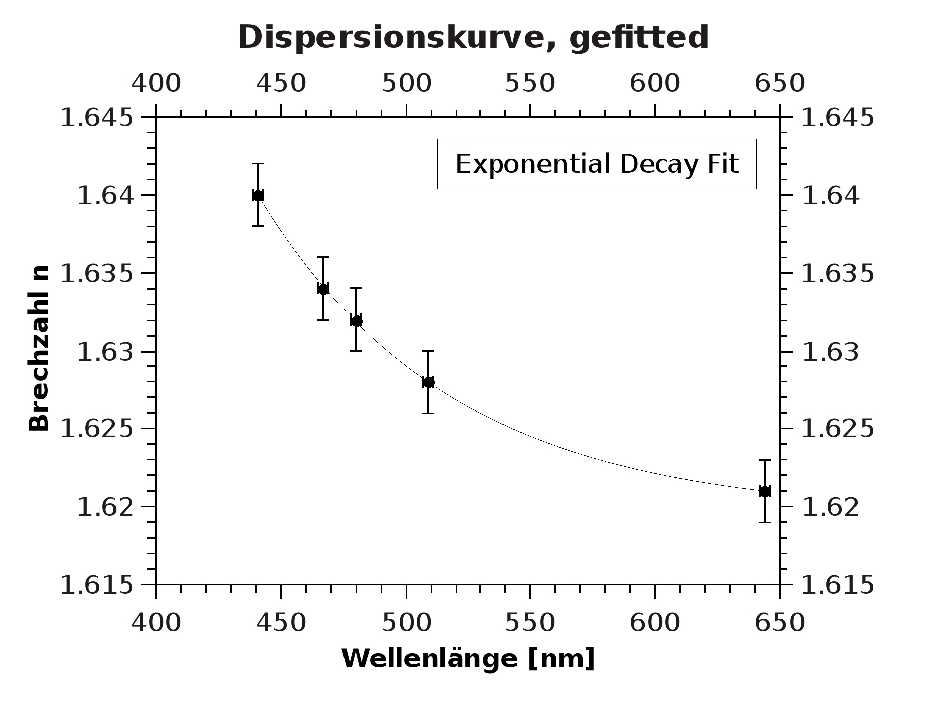
\includegraphics[scale=0.7]{fit.eps}
\end{figure}
\end{center}
Diese Kurve beschreibt unsere Messpunkte so gut, dass wir auf eine Ausgleichung mit der Cauchy-Gleichung verzichten können.
\subsection{Diskussion}
Wir verwenden trotz der Genauigkeit des Goniometers eine Unsicherheit von $\Delta\varphi_{min}$=5', da zwei weitere Ungenauigkeitsquellen beim Experimentieren hinzukommen: Einmal durch das Einstellen des Umkehrpunktes einer Spektrallinie auf die Mitte des Fadenkreuzes im Fernrohr, was eine Fingerspitzenangelegenheit ist. Und weiters, viel schwerwiegender, können wir beim Ablesen der Winkel durch die Lupe oft beide nicht genau erkennen, welche Grad-Markierung nun wirklich die richtige ist.\\
Die Unsicherheit der Brechungsindizes erhalten wir durch Größtfehlerabschätzung.\\
Die Wellenlänge des dunkelblauen Streifens war im Sensor nur schwach zu sehen, aber nach Abdunklung des Raumes, guter Ausrichtung des BLABLABLA und Hinein-zoomens doch zu erkennen.
Die Unsicherheit der Wellenlängenmessung wird aufgrund der Breite des Peaks mit 2nm angegeben.


\section{Lichtbrechung an einer planparallelen Platte}

\subsection{Aufgabenstellung}
Wir bestimmen die Brechung einer planparellelen Platte indem wir ihre scheinbare Dicke in einem Mikroskop betrachten und mit ihrer wirklichen, mit einer Mikrometerschraube gemessenen, vergleichen.
\subsection{Grundlagen}
Beim Durchgang eines Lichtstrahls durch eine transparente, planparallele Platte wird der Strahl parallel um die Distanz $\delta$ verschoben. Wenn AB die Strecke zwischen Eintritts und Austrittspunkt bedeutet, \textit{d} die tatsächliche Dicke der Platte, der Einfallswinkel $\varepsilon$ und der Brechungswinkel $\varepsilon '$, dann gilt:
\begin{gather*}
sin(\varepsilon-\varepsilon ') = \frac{\delta}{AB} \\
cos \varepsilon ' = \frac{d}{AB}  
\end{gather*}
\begin{equation}
\label{distanzdelta}
\delta =\frac{d\cdot sin(\varepsilon - \varepsilon ')}{cos\varepsilon '}
\end{equation}
Ist weiterhin BC die Distanz entlang dem Lot auf der Platte zwischen dem Austrittspunkt B und dem Schnittpunkt des verlängerten Eintrittsstrahles mit dem Lot der Punkt C, so scheint die Dicke der Platte um diese Distanz verringert. Ihre scheinbare Dicke \textit{b} entspricht der Differenz zwischen ihrer tatsächlichen Dicke \textit{d} und BC. Aus der Geometrie folgt die Brechzahl: 
\begin{equation}
\label{brechzahlplatte}
\frac{tan\varepsilon}{tan\varepsilon '}=\frac{d}{b}\approx\frac{sin\varepsilon}{sin\varepsilon '} = n
\end{equation}
\subsection{Versuchsaufbau und Methoden}
Wir verwenden ein Mikroskop im Durchlichtverfahren. Durch den Feintrieb der Hebung des Objektivtisches können wir den Abstand, um den wir die planparellele Platte heben müssen, damit wir von einem scharfen Bild auf der Oberseite zu einem scharfen Bild auf der Unterseite kommen, messen. Dieser Abstand ist die scheinbare Dicke \textit{b}. Wir messen sie an 5 verschiedenen Stellen und bilden den Mittelwert. Dann bestimmen wir die tatsächliche Dicke \textit{d} der Platte mit einer Mikrometerschraube. Aus (\ref{brechzahlplatte}) bestimmen wir dann die Brechzahl der Platte.
\subsection{Ergebnisse}
Scheinbare Dicke b:
Wir messen die scheinbare Dicke b durch Abzählen der Drehungen am Feintrieb des Mikroskops, bis der Strich auf der gegenüberliegenden Seite der Platte scharf im Bild erscheint, 5 mal:\\
\begin{center}


\begin{tabular}{|c|}

b\\
\hline
1.985mm\\
2.475mm\\
3.225mm\\
2.650mm\\
2.625mm\\
\end{tabular}
Der Mittelwert ist $\bar{b}$=(2.6 $\pm$ 0.2)mm
\end{center}

Wir messen die tatsächliche Dicke d mit der Mikrometerschraube und erhalten 3 mal den Messwert 3.27mm, 1 mal 3.26mm und 1 mal 3.28mm. Ihr Mittelwert ist

$$\bar{d}=(3.27 \pm 0.01) mm$$

Das Verhältnis aus d und b ergibt den Brechungsindex n:

$$\frac{d}{b}=n=1.3 \pm 0.1$$

\subsection{Diskussion}
Hierzu ist nicht viel zu sagen, außer dass es sehr mühsam war die Drehungen des Feintriebs am Mikroskop zu zählen und wir daher die große Abweichung der einzelnen Messwerte erklären.
\section{Refraktometrie}

\subsection{Aufgabenstellung}
Wir messen den Winkel der Totalreflexion mit einem Abbe-Refraktometer erst für sein Messprisma ohne Probeflüßigkeit, dann mit Probeflüßigkeit. Daraus berechnen wir die Brechungsindizes des Prismas \textit{N} und der Flüßigkeit \textit{n}. Schließlich messen wir den Brechungsindex \textit{n} direkt mit einem anderen Refraktometer. 
\subsection{Grundlagen}
Zuerst der Brechungsindex N des Messprismas. Hierbei verwenden wir den brechenden Winkel dieses Prismas, $\varphi$=61°.
\begin{equation}
\label{NMessprisma}
N=\sqrt{(\frac{cos\varphi + sin i}{sin \varphi})^2+1}
\end{equation}
i ist der Winkel der Totalreflexion ohne Probeflüßigkeit. \\
Daraus bekommen wir mit dem Winkel der Totalreflexion mit Probeflüßigkeit \textit{e}:
\begin{align}
\label{ns}
n=N \cdot sin e \\
sin i= N \cdot sin r \\
\varphi = r + e
\end{align}
n ist der Brechungsindex der Probeflüßigkeit, N der des Messprismas und e der Winkel 
\subsection{Versuchsaufbau und Methoden}
Wir verwenden ein Abbe-Refraktometer unter dem Licht einer Natriumdampflampe, das wir erst kalibrieren. Dann messen wir den Brechungsindex der Flüßigkeit direkt mit einem Handrefraktometer der Firma Krüss.
\subsection{Ergebnisse}
Wellenlänge des verwendeten Lichts: 590nm\\


Nullpunkt: 121°56' $\pm 1'$\\
\\
Winkel i ohne Flüßigkeit + Nullpunkt: 161°16'$\pm 1'$\\
\\
$\rightarrow$
Winkel i=39°40'$\pm 2'$\\
\\Winkel e mit Flüßigkeit + Nullpunkt:128°34'$\pm 1'$\\
\\
$\rightarrow$Winkel e=6°38'$\pm 2'$\\



Mit (\ref{NMessprisma}) erhalten wir für den Brechungsindex des Messprismas

$$ N = 1.624 \pm 0.0002 $$

und mit (\ref{ns}) 


$$ n = N \cdot \sin e = 0.20 \pm 0.03 $$

für den Brechungsindex der Flüßigkeit. \\

Direkt mit dem Handrefraktometer der Firma Krüss gemessen ergibt sich der Brechungsindex der Flüßigkeit zu:\\
\\n=1.357 $\pm$ 0.0005\\
\subsection{Diskussion}
Offensichtlich ist unser mit dem Abbe-Refraktometer gemessener Brechungsindex n falsch - er ist viel zu niedrig. Trotz mehrmaliger Rechnung und Überprüfung des Rechenwegs kommen wir zu keinem anderen Ergebnis. Wir vermuten, dass wir den Winkel e falsch gemessen haben - er ist es, dessen Sinus den Index so klein macht. 
\end{document}
